\chapter{Leistungsendstufen}
\section{Übernahmeverzerrung}

\begin{figure}[H]
    \centering
    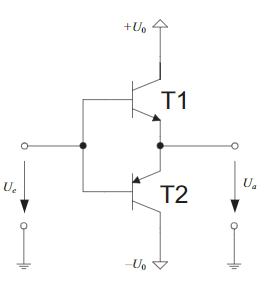
\includegraphics{tex/7_Leistungsverstaerker/pictures/Schematic_Emitterfolger.png}
    \caption{Push-Pull Endstufe}
    \label{fig:my_label}
\end{figure}

In diesem Kapitel werden Leistungsendstufen mit zwei komplementären Transistoren behandelt.

\begin{figure}[H]
    \centering
    \includegraphics[width = \textwidth]{simulations/7_Leistungsendstufe/Übernahmeverzerrungen.pdf}
    \caption{Übernahmeverzerrungen}
    \label{fig:my_label}
\end{figure}

Trotz der Unterschiede in der Signalform, waren für mich bei einer Grundfrequenz von \SI{1}{\hilo \hertz} keine Unterschiede hörbar.

Im Frequenzspektrum betrachtet, wirken sich diese nicht-Linearitäten  in der Verstärkung wie folgt aus:

\begin{figure}[H]
    \centering
    \includegraphics[width = \textwidth]{simulations/7_Leistungsendstufe/Übernahmeverzerrungen_fft.pdf}
    \caption{Übernahmeverzerrungen im Frequenzbereich}
\end{figure}

Man erkennt, dass besonders die ungeraden vielfachen der Grundfrequenz deutliche Oberwellen erzeugen (3, 5, 7 ... kHz).

\subsection{Warum gibt es keine Übernahmeverzerrungen bei hohem Lastwiderstand bzw. Leerlauf?Hinweis: siehe interne Beschaltung der Darlington–Transistoren}

Der verwendete NPN-Darlington-Transistor verfügt über eine leitende Verbindung zwischen Basis und Emitter ($R_1$ und $R_2$). Wenn die Transistoren sperren und am Emitter keine Last anliegt, wird der Emitter durch diese leitende Verbindung auf das Basisspannungspotential angehoben.

\begin{figure}[H]
    \centering
    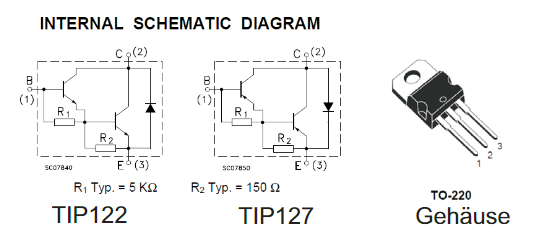
\includegraphics{tex/7_Leistungsverstaerker/pictures/Darlington.png}
    \caption{Interne Beschaltung der verwendeten Darlingtontransistoren}
\end{figure}

\section{Der rückgekoppelte Emitterfolger}

\begin{figure}[H]
    \centering
    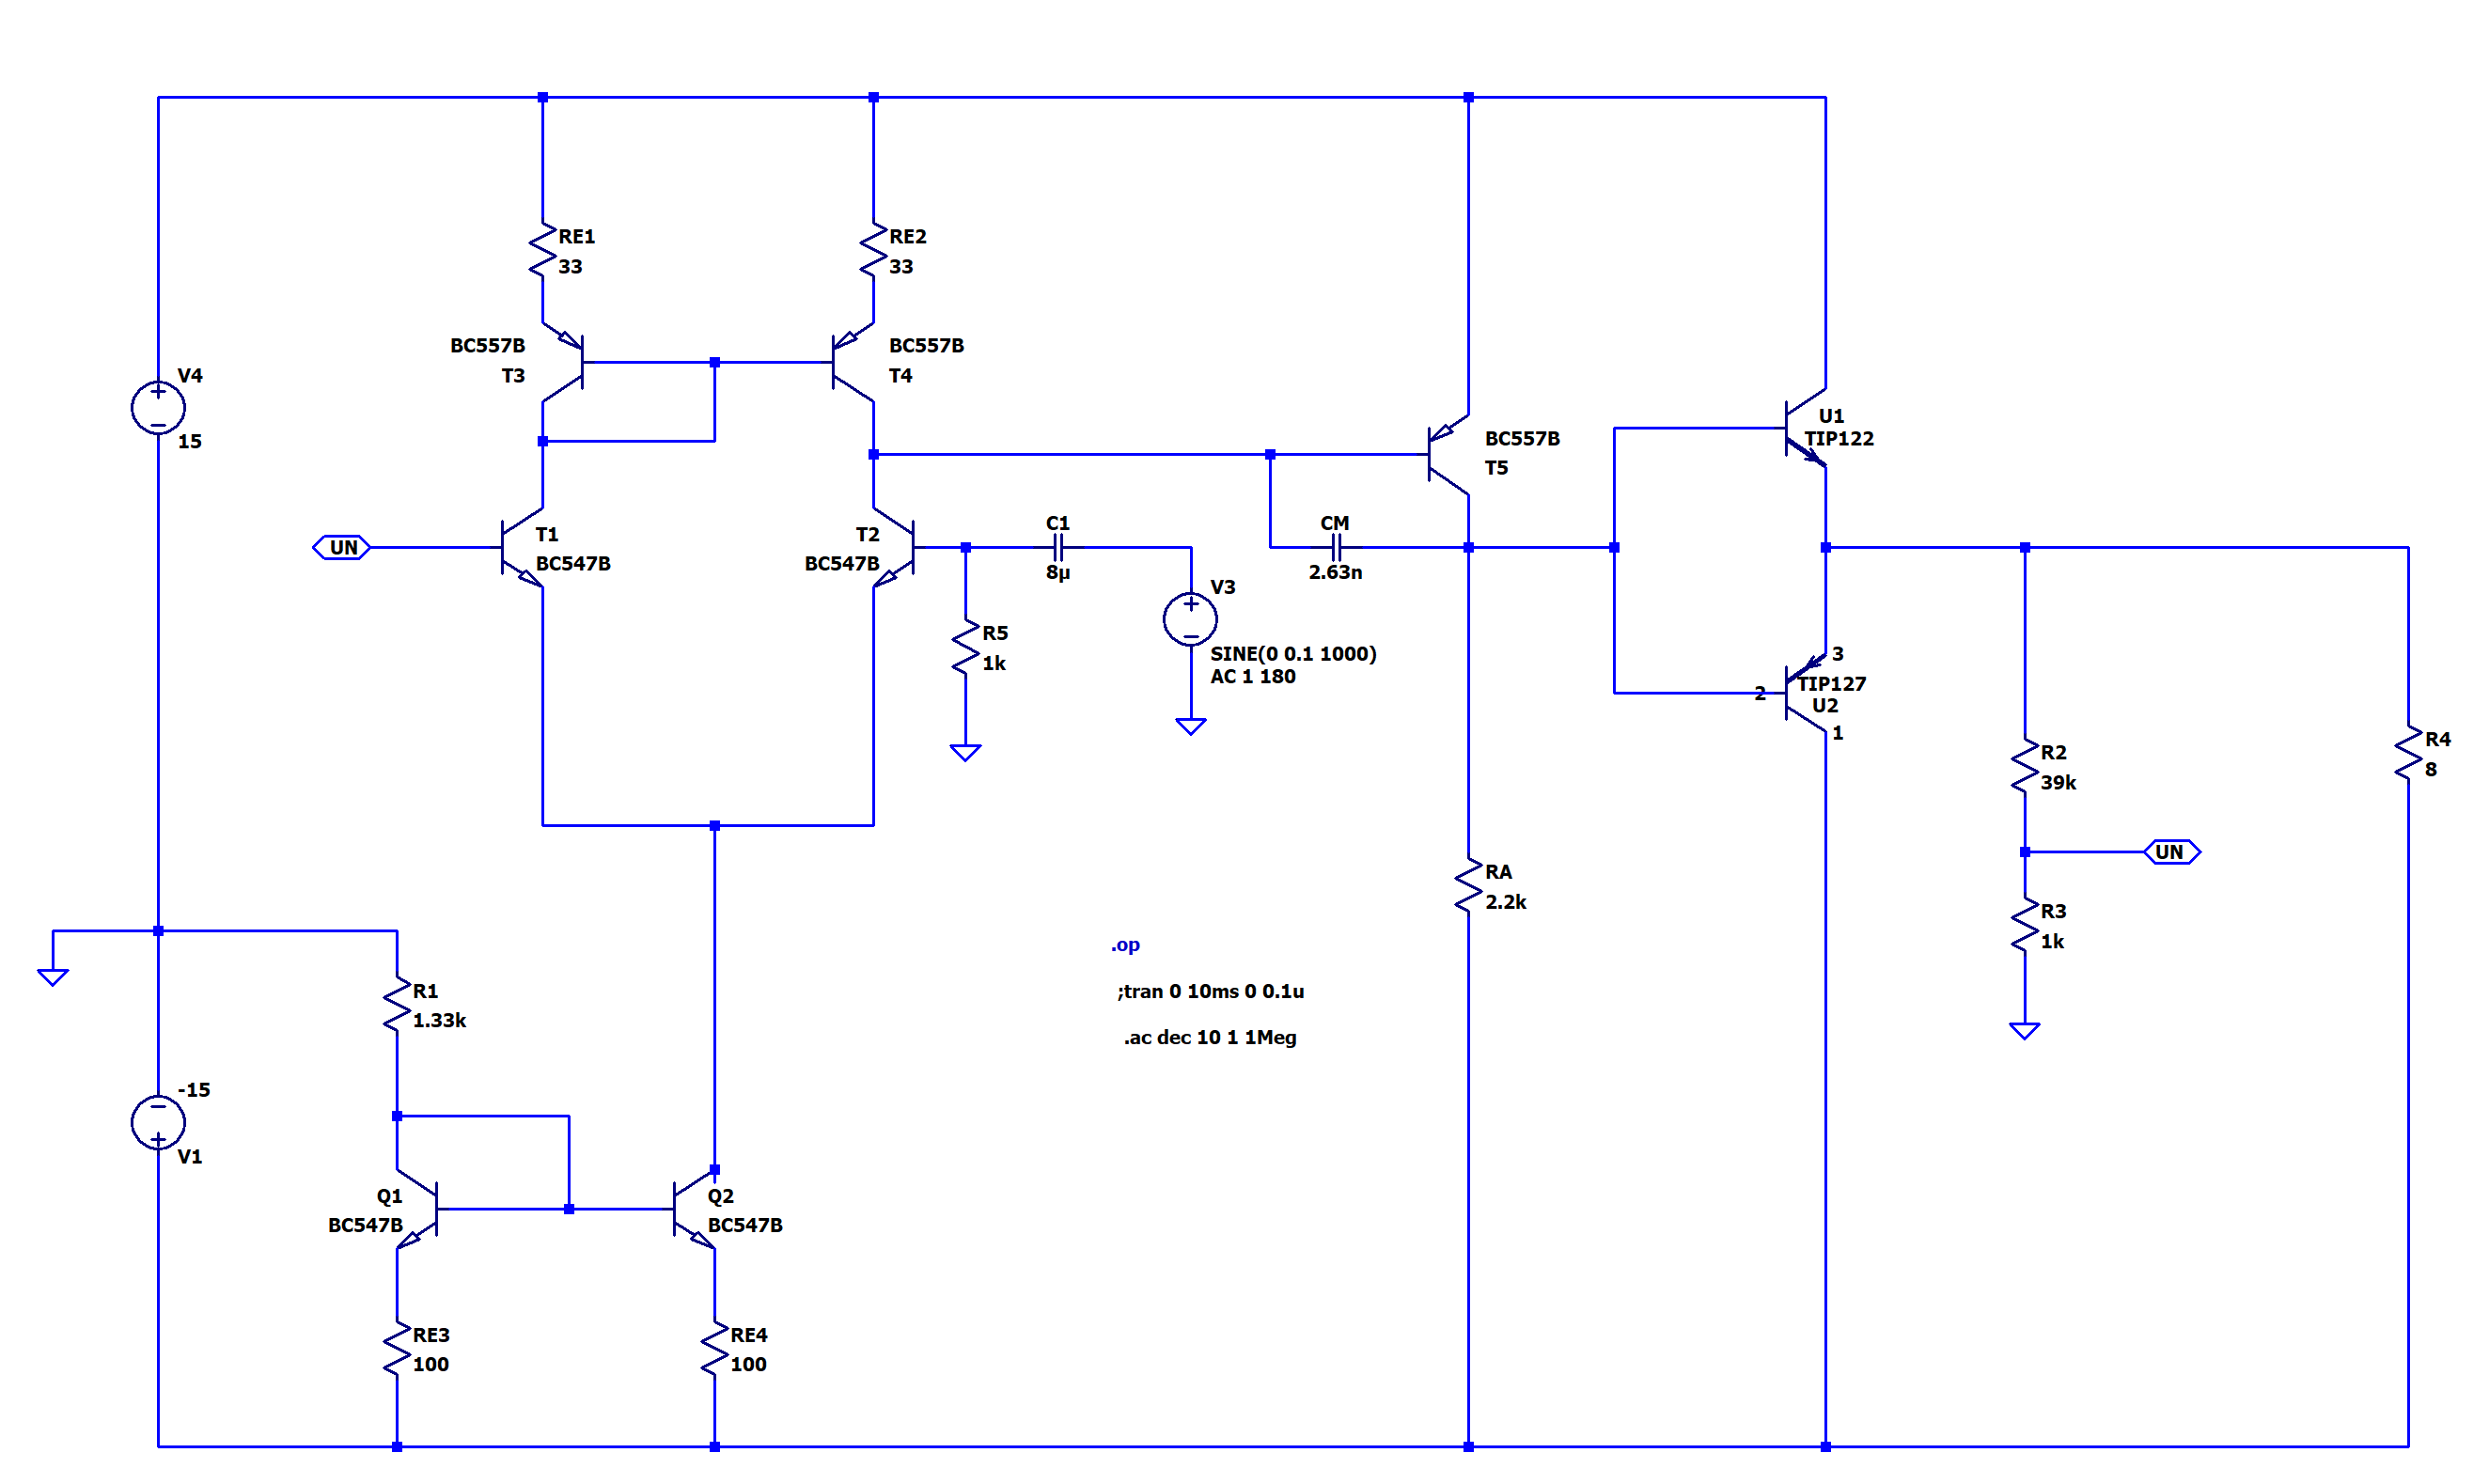
\includegraphics[width = \textwidth]{tex/7_Leistungsverstaerker/pictures/feedback_schem.png}
    \caption{Emitterfolger mit Feedback}
\end{figure}

\subsection{Dimensionierung Eingangshochpass und resultierender Amplitudengang}



\begin{equation}
    RC = \frac{1}{2 \pi \SI{20}{\hertz}} = \SI{7.958}{\milli \second} \rightarrow R = \SI{10}{\kilo \ohm}, C = \SI{8}{\micro \farad}
\end{equation}

\begin{figure}[H]
    \centering
    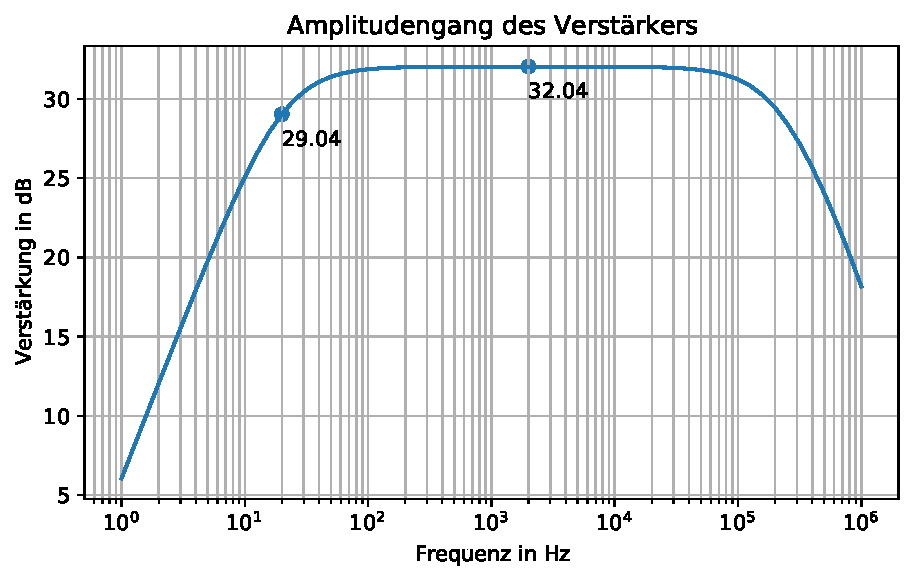
\includegraphics{tex/7_Leistungsverstaerker/pictures/Amplitudengang.pdf}
    \caption{Amplitudengang zwischen Eingang und Ausgang des Verstärkeres}
    \label{fig:my_label}
\end{figure}

Im Amplitudengang des Verstärkers ist deutlich zu erkennen, dass der Verstärker im Maximum bei circa \SI{20}{\kilo \hertz} um \SI{32}{dB} verstärkt. Das entspricht einer Verstärkung um den Faktor 40.
Bei einer Frequenz von \SI{20}{\hertz} wird um \SI{29}{dB} verstärkt, also die geforderten \SI{3}{dB} weniger durch den Hochpass am Eingang.

\subsection{Betrachtung der Linearität/Klirrfaktoren}

Es ist zu beurteilen wie sich die Klirrfaktoren dieser Schaltungen bei den Frequenzen \SI{1}{\kilo \hertz} und \SI{10}{\kilo \hertz} verhalten.

Der Ausgang des Verstärkers bewegt sich im Intervall $\left[\SI{-14.99}{\volt} \ldots \SI{13.23}{\volt}\right]$. Die maximale symmetrische Aussteuerung beträgt also $\pm \SI{13.23}{\volt}$

\begin{table}[H]
    \centering
    \begin{tabular}{|c||c||c|} \hline
         {Frequenz $f$} & {THD - $10\%$ Aussteuerung} & {THD -$80\%$ Aussteuerung} \\ \hline \hline
         \SI{1}{\kilo \hertz}& $0.0321\%$  & $0.038517\%$ \\ \hline
         \SI{10}{\kilo \hertz}& $0.020788\%$  & $0.035021\%$ \\ \hline
    \end{tabular}
    \caption{THD bei verschiedenen Aussteuerungsniveaus und Frequenzen}
    \label{tab:my_label}
\end{table}

Es zeigt sich also, dass Rückkopplung eine ausgezeichnete Methode ist um die Qualität der Verstärkung zu verbessern. Einerseits ist der Amplitudengang im relevanten Bereich sehr flach, andererseits ist auch die Nichtlinearität minimal.

\section{Gegentaktendstufe mit Ruhestromeinstellung}

\begin{figure}[H]
    \centering
    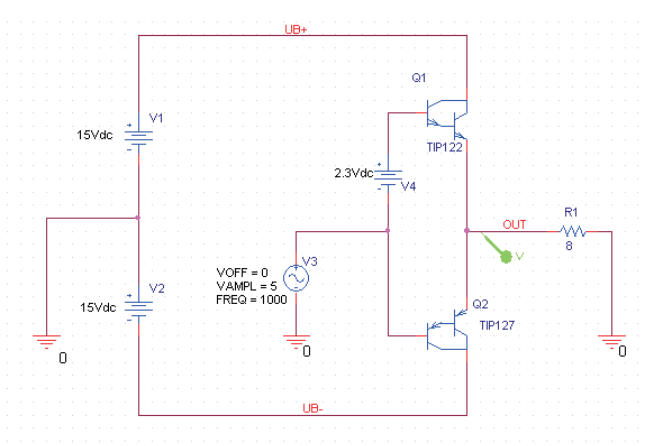
\includegraphics{tex/7_Leistungsverstaerker/pictures/Endstufe_Vorspannung_Schaltung.png}
    \caption{Endstufe mit Vorspannung}
    \label{fig:my_label}
\end{figure}

Wie bereits im Praktikumsskript thematisiert besteht in dieser Schaltung ein Trade-Off zwischen Linearität in der Verstärkung, dem Klirrfaktor und der Verlustleistung. Diese Verlustleisutngen treten nicht nur in den Transistoren, sondern auch im verwendeten Lautsprecher auf. Bei entsprechender Vorspannung erhält das Ausgangssignal einen DC-Offset, auch im Leerlauf wird Leistung in den Lautsprechern umgesetzt. Dies müsste durch eine Koppelkapazität behoben. 

\begin{table}[H]
    \centering
    \begin{tabular}{|c||c|c|}\hline
         $V_4$ & Total Harmonic Distortion & Querstrom im Leerlauf  \\ \hline \hline
         \SI{0}{\volt} (Referenz)& $11.33\%$ & \SI{32}{\micro \ampere} \\ \hline
         \SI{0.7}{\volt}& $7.39\%$ & \SI{32}{\micro \ampere} \\ \hline
         \SI{1.4}{\volt}& $3.54\%$ & \SI{199}{\micro \ampere} \\ \hline
         \SI{2.8}{\volt}& $0.06\%$ & \SI{1.4}{\ampere} \\ \hline
    \end{tabular} 
    \caption{verhalten bei verschiedenen Bias-Spannungen}
    \label{tab:my_label}
\end{table}

\section{Audioverstäker}

In dieser Aufgabe sollen die Punkte Biasing der Transistoren und Feedback kombiniert werden.

\begin{figure}[H]
    \centering
    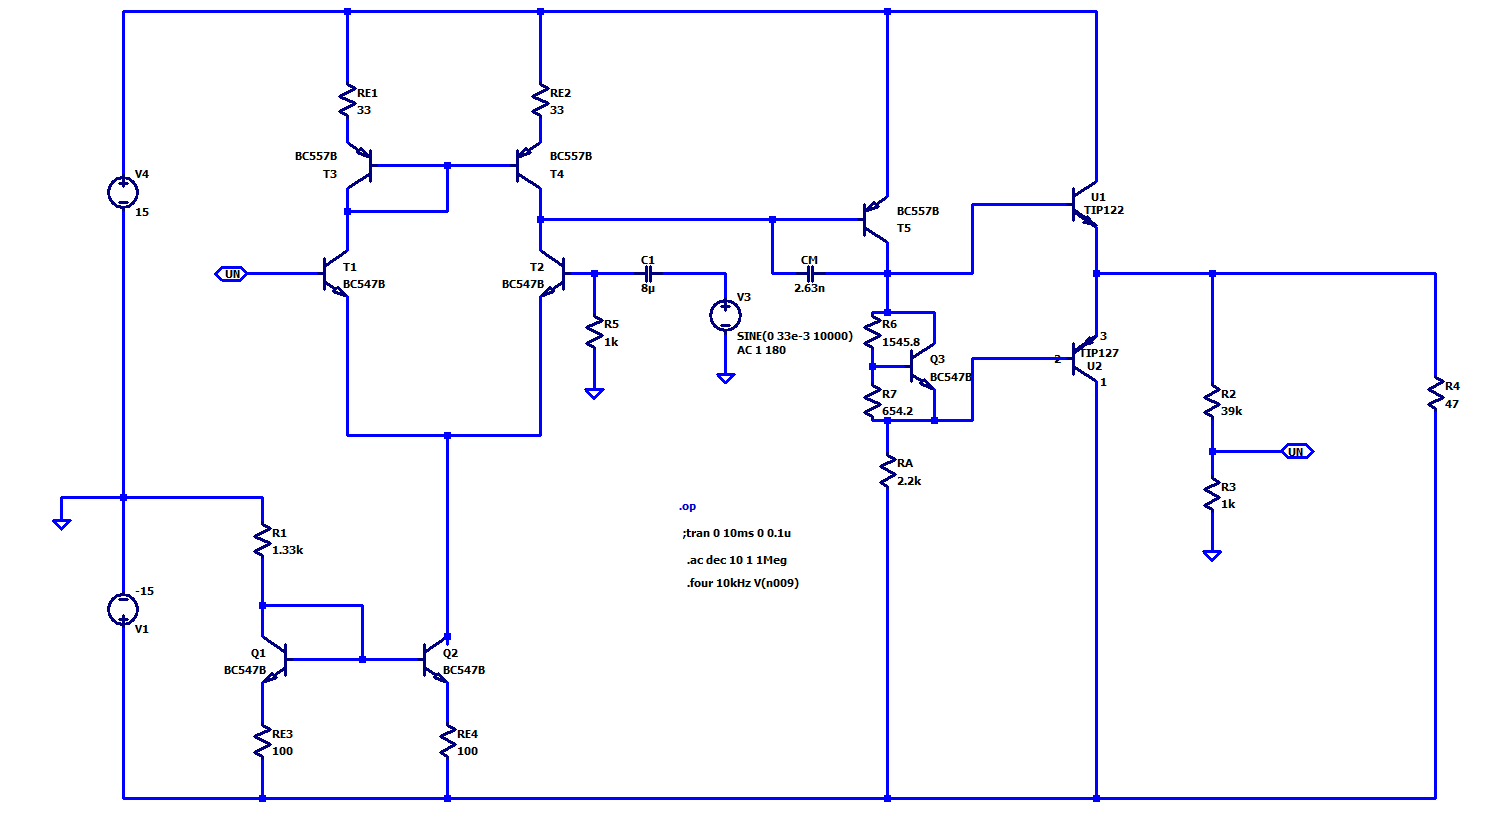
\includegraphics[width = \textwidth]{tex/7_Leistungsverstaerker/pictures/AudioAmp.png}
    \caption{Audioverstärker mit Biasing und Feedback}
\end{figure}

Das Vorspannnen der Transistoren wird über einen $U_{BE}$-Vervielfacher realisiert. Im Leerlauf (keine Aussteuerung und keine Last) sollte ein Querstrom von \SI{20}{\milli \ampere} fließen. Dies wird bei folgendem Verhältnis erreicht:

\begin{equation}
    \frac{R_6}{R_7} = \frac{\SI{1545.8}{\ohm}}{\SI{654.2}{\ohm}} = 2.36
\end{equation}

Die Spannung über diese \lgqq einstellbare Diode\rgqq{} beträgt also:

\begin{equation}
    U_{BE} \left( 1 + 2.36 \right) = U_{BE} 3.36 \approx \SI{2.35}{\volt}
\end{equation}

\subsection{Frequenzverhalten und Funktionalität}

Das Frequenzverhalten wird durch diese Modifikation nicht weiter verändert:

\begin{figure}[H]
    \centering
    \includegraphics{Audio}
    \caption{Amplitudengang zwischen Eingang und Ausgang des Verstärkeres (mit Feedback und Biasing)}
    \label{fig:my_label}
\end{figure}

\section{Der in Brücke geschaltete Verstärker}

\begin{figure}[H]
    \centering
    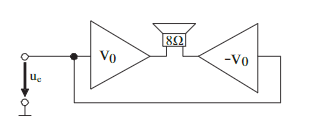
\includegraphics{tex/7_Leistungsverstaerker/pictures/Bridgeamp.png}
    \caption{Brückenschaltung mit 2 Verstärkern}
    \label{fig:my_label}
\end{figure}

Als abschließende Aufgabe ist zu Überlegen wie viel Leistung am Lautsprecher in dieser Konfiguration umgesetzt wird. Die Spannung am Lautsprecher wird effektiv verdoppelt, womit sich die umgesetzte Leistung vervierfachen müsste. 

\begin{equation*}
    P = \frac{(2 U)^2}{R} = 4 \frac{U^2}{R}
\end{equation*}